\subsection*{Lösungen zu Kapitel~\ref{kapitel:Drehstreckungen}: \emph{\embrace{Dreh-}Streckungen}}

\begin{proof}[Lösung zu Aufgabe~\ref{aufgabe:IMO2005_5}]
	Betrachte die Drehstreckung~$\sigma$  um $S$, die den Umkreis $\odot BCP$ auf den Umkreis $\odot DAP$ abbildet. Wir haben gesehen, dass~$\sigma$ auch als Projektion durch den zweiten Schnittpunkt der Umkreise beschrieben werden kann, also als Projektion durch~$P$. Weil~$P$ aber auch der Schnittpunkt von $AC$ und $BD$ ist, folgt $\sigma(C)=A$ und $\sigma(B)=D$. Also bildet $\sigma$ die Strecke $\overline{BC}$ auf die Strecke $\overline{DA}$ ab. Wegen $\abs*{BC}=\abs{DA}$ muss $\sigma$ somit eine Drehung sein.
	\begin{figure}[ht]
		\centering
		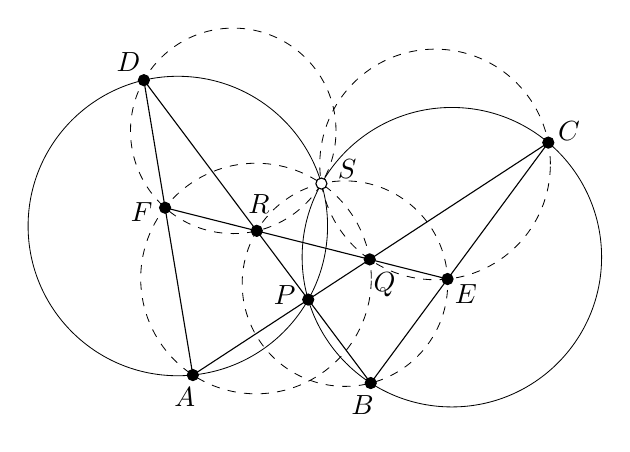
\begin{tikzpicture}[x=0.9cm,y=0.9cm]
			\draw[line width=0.3] (-0.826,0.977) circle (2.113);
			\draw[line width=0.3] (3.041,0.537) circle (2.113);
			\draw[line width=0.3,dashed] (-0.044,2.32) circle (1.45);
			\draw[line width=0.3,dashed] (2.804,1.846) circle (1.627);
			\draw[line width=0.3,dashed] (0.277,0.236) circle (1.627);
			\draw[line width=0.3,dashed] (1.532,0.164) circle (1.45);
			%\draw[line width=0.3,dashed] (1.014,-0.061) circle (0.824);
			\coordinate (A) at (-0.614,-1.126);
			\coordinate (B) at (1.896,-1.239);
			\coordinate (C) at (4.402,2.154);
			\coordinate (D) at (-1.305,3.035);
			\coordinate (E) at (2.98,0.229);
			\coordinate (F) at (-1.006,1.235);
			\coordinate (P) at (1.014,-0.061);
			\coordinate (Q) at (1.882,0.506);
			\coordinate (R) at (0.288,0.909);
			\coordinate (S) at (1.2,1.576);
			\draw (A) to (C) to (B) to (D) to cycle;
			\draw (E) to (F);
			\draw[fill=black] (A) circle (2pt) node[shift={(250:2ex)}] {$A$};
			\draw[fill=black] (B) circle (2pt) node[shift={(250:2ex)}] {$B$};
			\draw[fill=black] (C) circle (2pt) node[shift={(30:2ex)}] {$C$};
			\draw[fill=black] (D) circle (2pt) node[shift={(130:2ex)}] {$D$};
			\draw[fill=black] (E) circle (2pt) node[shift={(-40:2ex)}] {$E$};
			\draw[fill=black] (F) circle (2pt) node[shift={(190:2ex)}] {$F$};
			\draw[fill=black] (P) circle (2pt) node[shift={(170:2ex)}] {$P$};
			\draw[fill=black] (Q) circle (2pt) node[shift={(300:2.5ex)}] {$Q$};
			\draw[fill=black] (R) circle (2pt) node[shift={(85:2.25ex)}] {$R$};
			\draw[fill=white] (S) circle (2pt) node[shift={(30:2.5ex)}] {$S$};
		\end{tikzpicture}
	\end{figure}
	
	Aus $\abs*{BE}=\abs*{DF}$ folgt nun, dass $\sigma$ auch die Strecke $\overline{BE}$ auf die Strecke $\overline{DF}$ abbildet. Nach dem gleichen Argument wie für $\overline{BC}$ und $\overline{DA}$ wissen wir aber auch, dass es eine Drehung $\sigma'$ um den zweiten Schnittpunkt der Umkreise~$\odot BER$ und $\odot DFR$ gibt, die $\overline{BE}$ auf $\overline{DF}$ abbildet. Weil orientierungserhaltende Ähnlichkeitstransformationen durch~$2$ Punkte eindeutig bestimmt sind, muss $\sigma=\sigma'$ gelten. Folglich ist $S$ auch das Zentrum der Drehung~$\sigma'$ und liegt somit auf den Umkreisen $\odot BER$ und $\odot DFR$. Damit ist gezeigt, dass $BERS$ und $DFRS$ Sehnenvierecke sind. Das Argument für $CEQS$ und $AFQS$ geht analog. Damit ist~\ref{teilaufgabe:IMO2005_5a} gezeigt.
	
	Für~\ref{teilaufgabe:IMO2005_5b} machen wir eine Winkeljagd (und betrachten der Einfachheit halber nur den Lagebeziehungsfall aus der Skizze). Es gilt $\winkel RSQ=\winkel FSQ-\winkel FSR$. Nach dem Peripheriewinkelsatz im Sehnenviereck $FRSD$ gilt $\winkel FSR=\winkel FDR=\winkel ADP$. Andererseits gilt im Sehnenviereck $AQSF$ die Gleichung $\winkel FSQ=180^\circ-\winkel QAF=180^\circ-\winkel PAD$. Aus der Innenwinkelsumme im Dreieck $APD$ folgt nun
	\begin{equation*}
		\winkel RSQ=\winkel FSQ-\winkel FSR=\parens*{180^\circ-\winkel PAD}-\winkel ADP=\winkel DPA=180^\circ-\winkel QPR\,.
	\end{equation*}
	Damit ist $PQRS$ ein Sehnenviereck.
\end{proof}
\begin{proof}[Lösung zu Aufgabe~\ref{aufgabe:FermatPunkt}]
	Sei~$P$ der von~$C$ verschiedene Schnittpunkt der Umkreise $\odot BXC$ und $\odot CYA$. Dann gilt $\winkel BPC=180^\circ-60^\circ=120^\circ$ und $\winkel CPA=180^\circ-60^\circ=120^\circ$. Es folgt
	\begin{equation*}
		\winkel BZA+\winkel APB=60^\circ+\parens*{360^\circ-120^\circ-120^\circ}=180^\circ\,.
	\end{equation*}
	Also ist $AZBP$ ein Sehnenviereck und somit liegt~$P$ auch auf dem Umkreis~$\odot AZB$. Damit ist~\ref{teilaufgabe:FermatPunkt} bewiesen.
	
	\begin{figure}[ht]
		\centering
		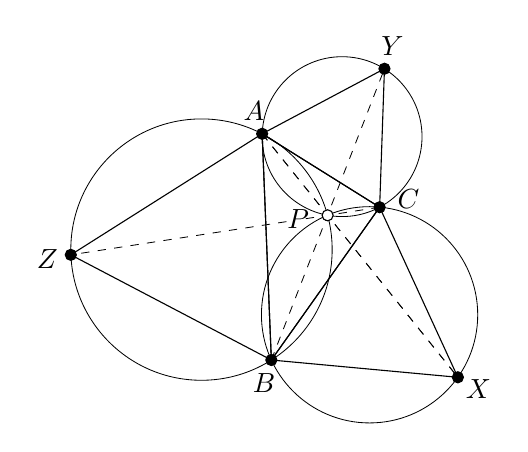
\begin{tikzpicture}[x=1.8cm,y=1.8cm]
			\draw[line width=0.3] (-0.257,0.201) circle (0.922);
			\draw[line width=0.3] (0.929,-0.259) circle (0.763);
			\draw[line width=0.3] (0.735,0.998) circle (0.564);
			\coordinate (A) at (0.171,1.018);
			\coordinate (B) at (0.236,-0.578);
			\coordinate (C) at (1,0.5);
			\coordinate (P) at (0.633,0.443);
			\coordinate (X) at (1.552,-0.7);
			\coordinate (Y) at (1.034,1.477);
			\coordinate (Z) at (-1.179,0.164);
			\draw (A) to (C) to (B) to (A) to (Z) to (B) to (X) to (C) to (Y) to (A) to cycle;
			\draw[line width=0.3,dashed] (A) to (X);
			\draw (A) to (C) to (B) to cycle;
			\draw[line width=0.3,dashed] (A) to (X);
			\draw[line width=0.3,dashed] (B) to (Y);
			\draw[line width=0.3,dashed,shorten >=-2ex] (C) to (P);
			\draw[line width=0.3,dashed,shorten <=3.5ex] (P) to (Z);
			\draw[fill=black] (A) circle (2pt) node[shift={(110:2ex)}] {$A$};
			\draw[fill=black] (B) circle (2pt) node[shift={(252:2ex)}] {$B$};
			\draw[fill=black] (C) circle (2pt) node[shift={(15:2.5ex)}] {$C$};
			\draw[fill=white] (P) circle (2pt) node[shift={(188:2.5ex)}] {$P$};
			\draw[fill=black] (X) circle (2pt) node[shift={(330:2ex)}] {$X$};
			\draw[fill=black] (Y) circle (2pt) node[shift={(70:2ex)}] {$Y$};
			\draw[fill=black] (Z) circle (2pt) node[shift={(190:2ex)}] {$Z$};
		\end{tikzpicture}
	\end{figure}
	
	Für~\ref{teilaufgabe:GeradenSchneidenSichImFermatPunkt} betrachte die Drehstreckung~$\sigma$ um~$A$, die~$Z$ auf~$C$ abbildet. Weil $AZB$ und $ACY$ gleichseitige Dreiecke sind, wird dann auch $B$ auf~$Y$ abgebildet. Dann werden auch die Umkreise $\odot AZB$ und $\odot CYA$ aufeinander abgebildet. Folglich lässt sich $\sigma$ aber auch als Projektion durch den zweiten Schnittpunkt~$P$ beschreiben. Wegen $\sigma(Z)=C$ und $\sigma(B)=Y$ muss~$P$ also auf $BY$ und auf~$CZ$ liegen. Analog liegt~$P$ auch auf $AX$.
\end{proof}
\begin{proof}[Lösung zu Aufgabe~\ref{aufgabe:SatzVonAubel}, Aufgabe~\ref{aufgabe:SatzVonAubelAufSteroiden} und zum Satz von Napoleon]
	Wir beweisen alle drei gleichzeitig, indem wir sie als Spezialfälle aus dem folgenden Master-Lemma folgern.
\end{proof}
\begin{satzmitnamen}[Master-Lemma für aufgesetzte Dreiecke]
	Sei $ABC$ ein Dreieck. Auf die Seiten $\overline{CA}$ und~$\overline{AB}$ werden nach außen Dreiecke $CYA$ und $AZB$ aufgesetzt. Dabei gelte $\winkel CAY=\winkel ZAB\eqqcolon\varphi$ sowie $\winkel YCA=\winkel ABZ\eqqcolon\psi$. Ferner sei $X$ ein Punkt, der bezüglich $BC$ in der gleichen Halbebene wie~$A$ liegt und für den $\winkel XCB=\winkel ZAB=\varphi$ sowie $\winkel CBX=\winkel ABZ=\psi$ gilt (das Dreieck $BCX$ wird also \emph{nicht} nach außen aufgesetzt). Sei $O$ der Mittelpunkt des Umkreises $\odot BCX$ und sei $P$ der Mittelpunkt des Umkreises $\odot AZB$. Dann ist das Dreieck $OYZ$ gleichschenklig mit Spitze~$O$ und außerdem ähnlich zum Dreieck $PAZ$.
\end{satzmitnamen}
\begin{proof}
	Betrachte die Drehstreckung~$\sigma$ mit Zentrum~$Z$, die $P$ auf $A$ abbildet. Wenn wir zeigen können, dass $\sigma(O)=Y$ ist, dann folgt wie gewünscht $OYZ\sim PAZ$. Ferner muss das Dreieck $PAZ$ gleichschenklig mit Spitze~$P$ sein, denn $P$ ist der Umkreismittelpunkt von $AZB$. Folglich wäre auch $OYZ$ gleichschenklig mit Spitze~$O$ und wir wären fertig.
	
	\begin{figure}[ht]
		\centering
		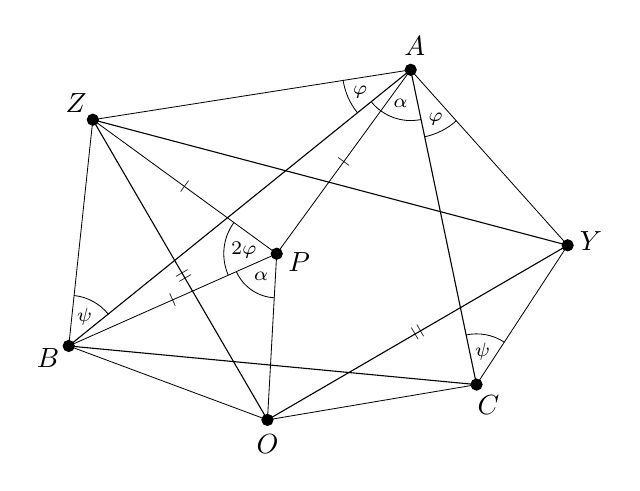
\begin{tikzpicture}[x=0.35cm,y=0.35cm]
			\coordinate (A) at (7.169,8.882);
			\coordinate (B) at (-5.239,-1.138);
			\coordinate (C) at (9.558,-2.54);
			\coordinate (X) at (1.972,-3.821);
			\coordinate (Y) at (12.864,2.515);
			\coordinate (Z) at (-4.364,7.071);
			\coordinate (O) at (2.308,2.209);
			\draw (A) to (B) to (C) to cycle;
			\draw [line width=0.3] (A) to node[sloped] {$\scriptscriptstyle|$} (O) to node[sloped] {$\scriptscriptstyle|$} (Z) to (A) to (Y) to (C) to (X) to (O) to node[sloped] {$\scriptscriptstyle|$} (B) to (Z) to (B) to (X);
			\draw (Z) to node[sloped,pos=0.52] {$\scriptscriptstyle||$} (X) to node[sloped] {$\scriptscriptstyle||$} (Y) to cycle;
			\begin{scriptsize}
				%\draw [line width=0.3, shift={(B)}] (-20.412:0.62cm) arc (-20.412:-5.412:0.62cm);
				%\draw [line width=0.3, shift={(B)}] (-20.412:0.67cm) arc (-20.412:-5.412:0.67cm);
				%\draw [line width=0.3, shift={(C)}] (174.588:5.125em) arc (174.588:189.588:5.125em);
				\path (C) to node {$\psi$} ++ (79.31:3em);
				\draw [line width=0.3, shift={(C)}] (56.81:2.3em) arc (56.81:101.81:2.3em);
				\path (A) to node {$\varphi$} ++ (296.81:5em);
				\draw [line width=0.3, shift={(A)}] (281.81:3.1em) arc (281.81:311.81:3.1em);
				\path (A) to node {$\varphi$} ++ (203.922:5em);
				\draw [line width=0.3, shift={(A)}] (188.922:3.1em) arc (188.922:218.922:3.1em);
				\draw[line width=0.3,shift={(A)}] (218.922:2.3em) arc (218.922:281.81:2.3em);
				\path (A) to node {$\alpha$} ++ (253.366:3.2em);
				\path (B) to node {$\psi$} ++ (61.422:3em);
				\draw [line width=0.3, shift={(B)}] (38.922:2.3em) arc (38.922:83.922:2.3em);
				\path (O) to node {$2\varphi$} ++ (173.922:3em);
				\draw [line width=0.3, shift={(O)}] (143.922:2.4em) arc (143.922:203.922:2.4em);
				\path (O) to node {$\alpha$} ++ (235.366:2.5em);
				\draw [line width=0.3, shift={(O)}] (203.922:2em) arc (203.922:266.81:2em);
			\end{scriptsize}
			\draw [fill=black] (A) circle (2pt) node[shift={(80:2ex)}] {$A$};
			\draw [fill=black] (B) circle (2pt) node[shift={(210:2ex)}] {$B$};
			\draw [fill=black] (C) circle (2pt) node[shift={(300:2ex)}] {$C$};
			\draw [fill=black] (X) circle (2pt) node[shift={(270:2ex)}] {$O$};
			\draw [fill=black] (Y) circle (2pt) node[shift={(10:2ex)}] {$Y$};
			\draw [fill=black] (Z) circle (2pt) node[shift={(135:2ex)}] {$Z$};
			\draw [fill=black] (O) circle (2pt) node[shift={(-20:2ex)}] {$P$};
		\end{tikzpicture}
	\end{figure}
	
	Um $\sigma(O)=Y$ zu zeigen, betrachten wir zunächst die Drehstreckung~$\tau$ um~$B$, die $C$ auf $A$ abbildet. Weil die Dreiecke $BCX$ und $BAZ$ nach Annahme gleichsinnig ähnlich sind, werden sie unter~$\tau$ aufeinander abgebildet. Dann werden auch ihre Umkreismittelpunkte~$P$ und~$O$ aufeinander abgebildet. Aus $\tau(O)=P$ und $\tau(C)=A$ folgt nun, dass $BOP$ und $BCA$ gleichsinnig ähnlich sind. Insbesondere ist $\winkel BPO=\winkel BAC\eqqcolon\alpha$. Nun gilt $\winkel ZAY=2\varphi+\alpha$. Nach dem Zentri-Peripheriewinkelsatz gilt $\winkel ZPB=2\varphi$. Also ist auch $\winkel ZPO=\winkel ZPB+\winkel BPO=2\varphi+\alpha$. Somit stimmen die Dreiecke $ZOP$ und $ZYA$ in einem Winkel überein.
	
	Aus der Ähnlichkeit $BOP\sim BCA$ folgt ferner $\abs*{OP}/\abs*{BP}=\abs*{CA}/\abs*{AB}$. Weil~$P$ der Umkreismittelpunkt von $AZB$ ist, gilt $\abs*{BP}=\abs*{ZP}$. Aus der Ähnlichkeit $CYA\sim AZB$ folgt außerdem $\abs*{CA}/\abs{AB}=\abs*{AY}/\abs*{AZ}$. Wir erhalten $\abs{OP}/\abs{ZP}=\abs{AY}/\abs{AZ}$. Somit stimmen die Dreiecke $ZOP$ und $ZYA$ nicht nur in einem Winkel, sondern auch im Verhältnis der anliegenden Seiten überein. Also sind sie ähnlich. Nach Definition von~$\sigma$ gilt $\sigma(P)=A$. Aus der Ähnlichkeit $ZOP\sim ZYA$ folgt nun auch $\sigma(O)=Y$ und wir sind fertig.
\end{proof}
\begin{proof}[Lösung zu Aufgabe~\ref{aufgabe:InAnkreis}]
	Betrachte die Streckung~$\sigma$ mit Zentrum~$A$, die~$\omega$ auf~$\omega_a$ abbildet. Das Bild von $D$ ist ein Punkt~$\sigma(D)$ auf $\omega_a$, sodass die Tangente an~$\omega$ in $\sigma(D)$ parallel zur Tangente an $\omega_a$ in $D$, also parallel zu $BC$ ist. Es gibt aber nur zwei Punkte auf $\omega_a$, für die das der Fall ist, nämlich $E$ (dessen Tangente genau $BC$ selbst ist) und den Punkt~$S$, der $E$ diametral gegenüber liegt. Offensichtlich kann nicht $\sigma(D)=E$ sein, sonst würde $BC$ auf sich selbst abgebildet werden und $\sigma$ wäre die Identitätsabbildung, was absurd ist, weil $\omega$ und $\omega_a$ auf verschiedenen Seiten von~$BC$ liegen. Also kommt nur $\sigma(D)=S$ in Frage und es folgt, dass $A$, $D$ und $S$ auf einer Geraden liegen. Analog lässt sich zeigen, dass $A$, $N$ und $E$ auf einer Geraden liegen.
\end{proof}

\begin{figure}[ht]
	\centering
	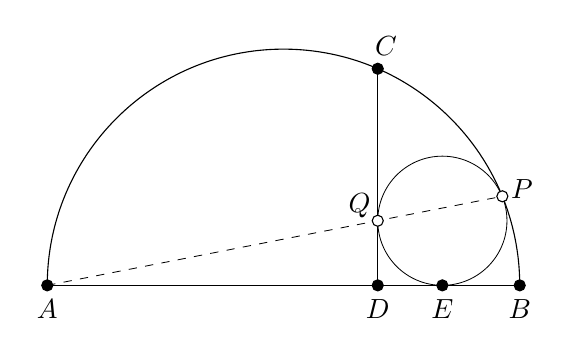
\begin{tikzpicture}[x=1.5cm,y=1.5cm]
		\draw (0:2) arc (0:180:2);
		\draw[line width=0.3] (1.345,0.547) circle (0.547);
		\coordinate (A) at (-2,0);
		\coordinate (B) at (2,0);
		\coordinate (C) at (0.798,1.834);
		\coordinate (D) at (0.798,0);
		\coordinate (E) at (1.345,0);
		\coordinate (P) at (1.853,0.754);
		\coordinate (Q) at (0.798,0.547);
		\draw (A) to (B);
		\draw (C) to (D);
		\draw[line width=0.3,dashed] (A) to (P);
		\draw[fill=black] (A) circle (2pt) node[shift={(270:2ex)}] {$A$};
		\draw[fill=black] (B) circle (2pt) node[shift={(270:2ex)}] {$B$};
		\draw[fill=black] (C) circle (2pt) node[shift={(70:2ex)}] {$C$};
		\draw[fill=black] (D) circle (2pt) node[shift={(270:2ex)}] {$D$};
		\draw[fill=black] (E) circle (2pt) node[shift={(270:2ex)}] {$E$};
		\draw[fill=white] (P) circle (2pt) node[shift={(20:1.75ex)}] {$P$};
		\draw[fill=white] (Q) circle (2pt) node[shift={(140:2ex)}] {$Q$};
	\end{tikzpicture}
\end{figure}
\begin{proof}[Lösung zu Aufgabe~\ref{aufgabe:551232}]
	Sei $P$ der Berührpunkt von $\omega$ mit $\Omega$ und sei $Q$ der Berührpunkt von~$\omega$ mit $\overline{CD}$. Nach dem Kreisberührungslemma sind $P$, $Q$ und $A$ kollinear und es gilt $\abs*{AP}\cdot\abs*{AQ}=\abs*{AC}^2$. Nach dem Sekanten-Tangentensatz gilt aber auch $\abs*{AP}\cdot \abs*{AQ}=\abs*{AE}^2$. Also ist $\abs*{AC}=\abs*{AE}$, wie behauptet.
\end{proof}
\begin{figure}[ht]
	\centering
	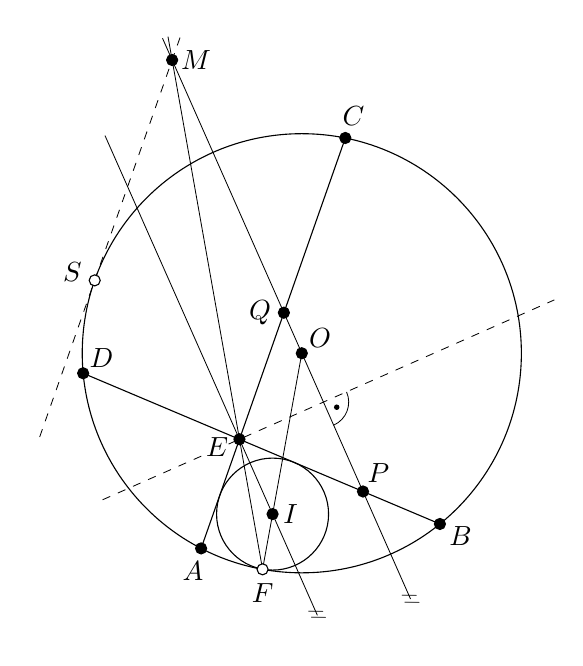
\begin{tikzpicture}[x=1.65cm,y=1.65cm]
		\clip (-2.09,-1.12) rectangle (1.97,3.58);
		\draw (0.02,1.074) coordinate (O) circle (1.69);
		\draw (-0.205,-0.164) coordinate (I) circle (0.431);
		\coordinate (A) at (-0.755,-0.428);
		\coordinate (B) at (1.083,-0.24);
		\coordinate (C) at (0.355,2.731);
		\coordinate (D) at (-1.663,0.92);
		\coordinate (E) at (-0.46,0.412);
		\coordinate (F) at (-0.282,-0.589);
		\coordinate (M) at (-0.978,3.331);
		\coordinate (P) at (0.491,0.01);
		\coordinate (Q) at (-0.118,1.386);
		\coordinate (S) at (-1.574,1.635);
		\draw (A) to (C);
		\draw (B) to (D);
		\draw[line width=0.3,dashed,shorten <=-1ex,shorten >=-0.25em] (E) to (1.915,1.463);
		\draw[line width=0.3,dashed,shorten <=3.5ex,shorten >=-2em] (E) to (-1.143,0.11);
		\draw[line width=0.3,shorten <=-2ex,shorten >=-4.25em] (M) to  node[pos=1.25,sloped] {$\scriptscriptstyle /\!/$} (P);
		\draw[line width=0.3,shorten <=-2ex,shorten >=-6em,dashed] (M) to (S);
		\draw[line width=0.3,shorten <=-2ex] (M) to (F);
		\draw[line width=0.3] (F) to (O);
		\draw[line width=0.3,shorten <=-12em,shorten >=-4em] (E) to  node[pos=2.35,sloped] {$\scriptscriptstyle /\!/$} (I);
		\draw[line width=0.3,shift={(0.187,0.698)}] (293.866:0.32cm) arc (293.866:383.866:0.32cm);
		\fill[black,shift={(0.187,0.698)}] (338.866:0.18cm) circle (1pt);
		\draw[fill=black] (A) circle (2pt) node[shift={(250:2ex)}] {$A$};
		\draw[fill=black] (B) circle (2pt) node[shift={(330:2ex)}] {$B$};
		\draw[fill=black] (C) circle (2pt) node[shift={(70:2ex)}] {$C$};
		\draw[fill=black] (D) circle (2pt) node[shift={(40:2ex)}] {$D$};
		\draw[fill=black] (E) circle (2pt) node[shift={(200:2ex)}] {$E$};
		\draw[fill=white] (F) circle (2pt) node[shift={(270:2ex)}] {$F$};
		\draw[fill=black] (I) circle (2pt) node[shift={(0:1.5ex)}] {$I$};
		\draw[fill=black] (M) circle (2pt) node[shift={(0:2ex)}] {$M$};
		\draw[fill=black] (O) circle (2pt) node[shift={(40:2ex)}] {$O$};
		\draw[fill=black] (P) circle (2pt) node[shift={(50:2ex)}] {$P$};
		\draw[fill=black] (Q) circle (2pt) node[shift={(180:2ex)}] {$Q$};
		\draw[fill=white] (S) circle (2pt) node[shift={(160:2ex)}] {$S$};
	\end{tikzpicture}
\end{figure}
\begin{proof}[Lösung zu Aufgabe~\ref{aufgabe:JuMaKlausur2014}]
	Wir bemerken zuerst, dass die Bedingung $\abs*{EP}=\abs*{EQ}$ dazu äquivalent ist, dass $\ell$ die Senkrechte von $O$ auf die Winkelhalbierende von $\winkel BEC$ ist. Sei~$I$ der Mittelpunkt von~$\omega$. Dann ist $EI$ die Winkelhalbierende von $AEB$. Weil $\winkel AEB$ und $\winkel BEC$ Nebenwinkel sind, steht $EI$ ebenfalls senkrecht auf der Winkelhalbierenden von $\winkel BEC$. Es folgt $EI\parallel \ell$.
	
	Betrachte nun die Streckung~$\sigma$ am Berührpunkt~$F$, die~$\omega$ auf~$\Omega$ abbildet. Dann bildet~$\sigma$ auch die Mittelpunkte dieser Kreise aufeinander ab, sodass $\sigma(I)=O$ sein muss. Also bildet~$\sigma$ die Gerade $EI$ auf die Parallele zu $EI$ durch~$O$ ab. Aus unserer obigen Beobachtung folgt somit $\sigma(EI)=\ell$. Als Schnittpunkt von $EF$ mit~$\ell$ muss $M$ folglich das Bild von~$E$ unter der Streckung~$\sigma$ sein.
	
	Das Bild von $AC$ unter~$\sigma$ ist eine Parallele zu $AC$, die den Kreis~$\Omega$ berührt. Weil $E$ auf $AC$ liegt, muss $\sigma(E)=M$ auf $\sigma(AC)$ liegen. Also berührt die Parallele zu $AC$ durch $M$ in der Tat den Kreis~$\Omega$.
\end{proof}